\documentclass[xcolor=dvipsnames,10pt]{beamer}
\usetheme{Boadilla}
\useinnertheme{rectangles}
\useoutertheme{infolines}
%\usecolortheme{dolphin}

\title[MFE]{
  Towards a Maude Formal Environment
}

\author[Dur\'an, Rocha, \'Alvarez]{
  Francisco Dur\'an\inst{1} \and Camilo Rocha\inst{2} \and Jos\'{e} M. \'Alvarez\inst{1}
}

\institute[UMA, U of I]{
  \inst{1}Universidad de M\'alaga \\
  \inst{2}University of Illinois at Urbana-Champaign
}

\date[FHCT 2011]{
  \\
  Festschrift Carolyn Talcot \\
  November 2011 \\
  Menlo Pak, CA
}

\newcommand{\enfa}[1]{{\color{Red}#1}}

\newcommand{\csuea}[2]{{\rm CSU}_{#2}(#1)}
\newcommand{\vind}{\vdash_{\rm ind}}
\newcommand{\rcal}{\mathcal{R}}
\newcommand{\kcal}{\mathcal{K}}
\newcommand{\mcal}{\mathcal{M}}
\newcommand{\tcal}{\mathcal{T}}
\newcommand{\acal}{\mathcal{A}}
\newcommand{\ecal}{\mathcal{E}}
\newcommand{\ecalpi}{\mathcal{E}_\Pi}
\newcommand{\reach}{{\rm reach}}
\newcommand{\states}{\mathfrak{s}}
\newcommand{\iffo}{\Longleftrightarrow}
\newcommand{\mimps}{\Longrightarrow}
\newcommand{\imps}{\Rightarrow}
\newcommand{\rews}{\rightarrow}
\newcommand{\rewsn}[1]{\stackrel{#1}{\rews}}
\newcommand{\true}{\top}
\newcommand{\false}{\bot}
\newcommand{\eq}[2]{#1 = #2}
\newcommand{\ceq}[3]{#1 = #2 \; {\rm if} \; #3}
\newcommand{\qeq}[3]{(\forall #1) \; #2 = #3}
\newcommand{\qceq}[4]{(\forall #1) \; #2 = #3 \; {\rm if} \; #4}
\newcommand{\rl}[2]{#1 \rews #2}
\newcommand{\crl}[3]{#1 \rews #2 \; {\rm if} \; #3}
\newcommand{\qrl}[3]{(\forall #1) \; #2 \rews #3}
\newcommand{\qcrl}[4]{(\forall #1) \; #2 \rews #3 \; {\rm if} \; #4}
\newcommand{\qrln}[4]{(\forall #1) \; #2 \rewsn{#4} #3}
\newcommand{\qcrln}[5]{(\forall #1) \; #2 \rewsn{#5} #3 \; {\rm if} \; #4}

\begin{document}

\begin{frame}
  \titlepage
\end{frame}

%%%%%%%%%%%%%%%%%%%%%%%%%%%%%%%%%%%%%%%%%%%%%%%%%%%%%%%%%%%%%%%%%%%%%%%%%%%%%%%%%%%%%%%
\section{Introduction}

%%%%%%%%%%%%%%%%%%%%%%%%%%%%%%%%%%%%%%%%%%%%%%%%%%%%%%%%%%%%%%%%%%%%%%%%%%%%%%%%%%%%%%%
\begin{frame}
  \frametitle{Maude's formal environment}
  
%These frames present the main features of several tools concerned with the analysis of either Maude specifications: the ITP, MTT, CRC, ChC, and SCC tools. These tools, together with Maude itself and its searching and model-checking capabilities, constitute Maude?s formal environment.

\begin{center}
\includegraphics[width=\textwidth]{tools-figures/formal-tool-env-1}
\end{center}

\end{frame}
%%%%%%%%%%%%%%%%%%%%%%%%%%%%%%%%%%%%%%%%%%%%%%%%%%%%%%%%%%%%%%%%%%%%%%%%%%%%%%%%%%%%%%%
\begin{frame}
  \frametitle{Maude's formal environment: part of Maude or around it}
  
\begin{center}
\includegraphics[width=\textwidth]{tools-figures/formal-tool-env-2}
\end{center}

\end{frame}
%%%%%%%%%%%%%%%%%%%%%%%%%%%%%%%%%%%%%%%%%%%%%%%%%%%%%%%%%%%%%%%%%%%%%%%%%%%%%%%%%%%%%%%
\begin{frame}
  \frametitle{Maude's formal environment: tools around Maude}
  
\begin{center}
\includegraphics[width=\textwidth]{tools-figures/formal-tool-env-3}
\end{center}

\end{frame}
%%%%%%%%%%%%%%%%%%%%%%%%%%%%%%%%%%%%%%%%%%%%%%%%%%%%%%%%%%%%%%%%%%%%%%%%%%%%%%%%%%%%%%%

\begin{frame}
  \frametitle{Maude and its formal environment (MFE)}

  \begin{itemize}
    \item Maude is a declarative language and system based on 
rewriting logic in which computation
corresponds to efficient deduction by rewriting.

    \item Several tools for verifying properties of Maude specifications available.

    \item These tools work in isolation, 
making it inconvenient to switch between their environments
and difficult to exchange data between them.

    \item MFE is
an executable and \enfa{highly extensible} software infrastructure
within which a user can \enfa{interact} with several 
tools to mechanically verify properties of Maude specifications.

    \item In MFE, tool \enfa{interoperability} allows for discharging proof obligations
of different nature without switching between different
tool environments.
  \end{itemize}
\end{frame}

%%%%%%%%%%%%%%%%%%%%%%%%%%%%%%%%%%%%%%%%%%%%%%%%%%%%%%%%%%%%%%%%%%%%%%%%%%%%%%%%%%%%%%%

\begin{frame}[fragile]
  \frametitle{Motivation}
  \framesubtitle{The Example of Readers and Writers}

We want to check that it is never the case that
  	\begin{description}
	\item[(i)] more than one writer or 
	\item[(ii)] writers and readers 
	\end{description}
share a critical resource at the same time. 

\bigskip

\begin{minipage}{0.45\linewidth}
{
\scriptsize
\begin{verbatim}
  fmod MNAT is
    sort MNat .
    op 0 : -> MNat [ctor] .
    op s : MNat -> MNat [ctor] .
  endfm 
\end{verbatim}
}
\end{minipage}
\begin{minipage}{0.45\linewidth}
{
\scriptsize
\begin{verbatim}
  mod READERS-WRITERS is
    protecting MNAT .
    sort Config .
    op <_,_> : MNat MNat -> Config [ctor] .
    vars R W : MNat .
    rl [wrt+] : < 0, 0 > => < 0, s(0) > .
    rl [wrt-] : < R, s(W) > => < R, W > .
    rl [rdr+] : < R, 0 > => < s(R), 0 > .
    rl [rdr-] : < s(R), W > => < R, W > .
  endm 
\end{verbatim}
}
\end{minipage}
\end{frame}

%%%%%%%%%%%%%%%%%%%%%%%%%%%%%%%%%%%%%%%%%%%%%%%%%%%%%%%%%%%%%%%%%%%%%%%%%%%%%%%%%%%%%%%

\begin{frame}
  \frametitle{The Maude Formal Environment (MFE)}

  An \enfa{executable formal specification in Maude}
  within which a user can interact with tools to mechanically verify properties
  of Maude specifications:

  \begin{itemize}
    \item It has been designed to be easily extended with tools having
      \enfa{heterogeneous designs}.

    \begin{itemize}
      \item It currently offers five tools.
    \end{itemize}

    \item It implements a \enfa{mechanism to keep track of pending proof
      obligations}.

    \item Its \enfa{tool interoperability} allows for discharging proof obligations of
      different nature without switching between different tool environments
      and presents the user with \enfa{a consistent user interface}.

    \item It allows the execution of several instances of each tool.

  \end{itemize}
\end{frame}

%%%%%%%%%%%%%%%%%%%%%%%%%%%%%%%%%%%%%%%%%%%%%%%%%%%%%%%%%%%%%%%%%%%%%%%%%%%%%%%%%%%%%%%

%\begin{frame}
%  \frametitle{Its design and implementation}

%  \begin{itemize}
%    \item MFE is modeled as an object-based system in which the tools are 
%objects and their communication mechanism
%is message passing. 

%    \item The MFE design is highly extensible and amenable to tool interoperability.

%    \item It has been designed to be easily extended with tools having
%      heterogeneous designs.
%      
%    \item The use of patterns such as the {\em model-view-controller} 
%pattern allows us to maximize reuse and simplify interaction and addition of further tools. 

%  \end{itemize}
%\end{frame}

%%%%%%%%%%%%%%%%%%%%%%%%%%%%%%%%%%%%%%%%%%%%%%%%%%%%%%%%%%%%%%%%%%%%%%%%%%%%%%%%%%%%%%%

%\begin{frame}
%  \frametitle{Motivation}
%  \framesubtitle{The Example of Readers and Writers}

%  \begin{itemize}
%    \item {\tt R+W} needs to be executable, i.e., its equations ground
%      Church-Rosser and terminating, and its rewrite rules ground coherent
%      with respect the equations
%    \item for initial state $\langle 0,0\rangle$, the set of initial states
%      is infinite, so we apply a state abstraction in {\tt R+W-ABS} which
%      needs to be checked executable
%  \end{itemize}
%\end{frame}

%%%%%%%%%%%%%%%%%%%%%%%%%%%%%%%%%%%%%%%%%%%%%%%%%%%%%%%%%%%%%%%%%%%%%%%%%%%%%%%%%%%%%%%
%\begin{frame}
%  \frametitle{Outline}
%  \tableofcontents
%\end{frame}

%%%%%%%%%%%%%%%%%%%%%%%%%%%%%%%%%%%%%%%%%%%%%%%%%%%%%%%%%%%%%%%%%%%%%%%%%%%%%%%%%%%%%%%
%\section{Tools in the Environment}

%%%%%%%%%%%%%%%%%%%%%%%%%%%%%%%%%%%%%%%%%%%%%%%%%%%%%%%%%%%%%%%%%%%%%%%%%%%%%%%%%%%%%%%
%\begin{frame}
%  \frametitle{Outline}
%  \tableofcontents[currentsection]
%\end{frame}

%%%%%%%%%%%%%%%%%%%%%%%%%%%%%%%%%%%%%%%%%%%%%%%%%%%%%%%%%%%%%%%%%%%%%%%%%%%%%%%%%%%%%%%
\begin{frame}
  \frametitle{Tool Overview}

  In the current version of MFE one can interact with the following tools:

  \begin{description}
    \item[MTT] {\em Maude Termination Tool}
      
      termination of equational and rewrite specifications

    \item[SCC] {\em Sufficient Completeness Checker}
      
      sufficient completeness and freeness of equational specifications,
      and deadlock of rewrite specifications

    \item[CRC] {\em Church-Rosser Checker}
      
      ground confluence and sort-decreasingness of equational specifications

    \item[ChC] {\em Maude Coherence Checker}
      
      ground coherence of rewrite specifications

    \item[ITP] {\em Inductive Theorem Prover}
      
      inductive properties of equational specifications

  \end{description}
\end{frame}

%%%%%%%%%%%%%%%%%%%%%%%%%%%%%%%%%%%%%%%%%%%%%%%%%%%%%%%%%%%%%%%%%%%%%%%%%%%%%%%%%%%%%%%
\begin{frame}
  \frametitle{Tool-dependency Graph in MFE}

  One important aspect in the integration task is the interaction complexity due to the
  nontrivial dependencies among tools

  \begin{center}
    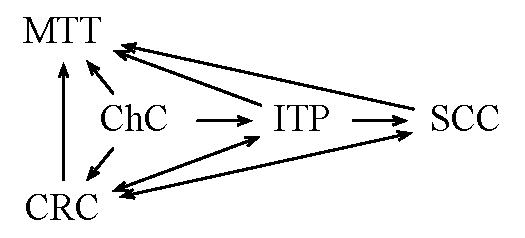
\includegraphics[width=6cm]{tool-dep}
  \end{center}
\end{frame}

%%%%%%%%%%%%%%%%%%%%%%%%%%%%%%%%%%%%%%%%%%%%%%%%%%%%%%%%%%%%%%%%%%%%%%%%%%%%%%%%%%%%%%%
\section{Design and Main Features}

%%%%%%%%%%%%%%%%%%%%%%%%%%%%%%%%%%%%%%%%%%%%%%%%%%%%%%%%%%%%%%%%%%%%%%%%%%%%%%%%%%%%%%%
%\begin{frame}
%  \frametitle{Outline}
%  \tableofcontents[currentsection]
%\end{frame}

%%%%%%%%%%%%%%%%%%%%%%%%%%%%%%%%%%%%%%%%%%%%%%%%%%%%%%%%%%%%%%%%%%%%%%%%%%%%%%%%%%%%%%%
\begin{frame}
  \frametitle{MFE Design Overview}

  \begin{itemize}
    \item MFE is modeled in Maude as an interactive \enfa{object-based system} where
      \begin{itemize}
        \item tools are objects, 
        \item the communication mechanism is message passing, and
        \item user interaction is available through Full Maude.
      \end{itemize}
    \item Integration and interoperation of tools within MFE is module-centric
      given that its main purpose is to support formal analysis of Maude modules.
    \item Although some classes and functionality are provided in MFE, it imposes
      no constraint on how each tool should model its particular domain or maintains
      its internal state.
    \item The use of patterns such as the {\em model-view-controller} 
pattern allows us to \enfa{maximize reuse and simplify interaction} and addition of further tools. 

  \end{itemize}
\end{frame}

%%%%%%%%%%%%%%%%%%%%%%%%%%%%%%%%%%%%%%%%%%%%%%%%%%%%%%%%%%%%%%%%%%%%%%%%%%%%%%%%%%%%%%%
\begin{frame}[fragile]
  \frametitle{Main Classes}

  The object-oriented model of MFE consists of three main classes

  \begin{description}
    \item[\texttt{  \small Proof}] proof objects that keep the state of specific proof requests
    \item[\texttt{  \small Tool}] tool objects that keep the life-cycle of proof objects
    \item[\texttt{  \small Controller}] provides a centralized entry point for handling user request
  \end{description}

\smallskip

\begin{center}
\includegraphics[width=.65\textwidth]{tools-figures/mfe-classes.png}
\end{center}

\end{frame}

%%%%%%%%%%%%%%%%%%%%%%%%%%%%%%%%%%%%%%%%%%%%%%%%%%%%%%%%%%%%%%%%%%%%%%%%%%%%%%%%%%%%%%%
\begin{frame}[fragile]
  \frametitle{User Interaction}

  The user interacts with the environment via commands
\smallskip
\begin{minipage}{0.45\linewidth}
  \begin{itemize}
    \item each command is encapsulated as a message in the object configuration
    \item each tool object and the controller object have a module defining the
      signature of commands it can handle
%    \begin{itemize}
%      \item the controller handles any command it can parse
%      \item if the controller receives a command it cannot parse, then it delegates
%        the message to the {\em active} tool
%      \item if the tool can parse the delegated command, then it notifies the controller
%        and handles the command
%      \item otherwise, it will notify the failure to the controller, which in turn
%        will output an error message to the user
%    \end{itemize}
  \end{itemize}
\end{minipage}
%\smallskip
\begin{minipage}{0.45\linewidth}
\begin{center}
\includegraphics[width=\textwidth]{tools-figures/mfe-structure.png}
\end{center}
\end{minipage}
\end{frame}

%%%%%%%%%%%%%%%%%%%%%%%%%%%%%%%%%%%%%%%%%%%%%%%%%%%%%%%%%%%%%%%%%%%%%%%%%%%%%%%%%%%%%%%
%\begin{frame}
%  \frametitle{Commands in MFE}
%  
%  MFE provides the following user commands:

%  \begin{description}
%    \item[\texttt{  \small(select tool <tool-name> .)}]
%      %\noindent \texttt{  \small(select tool <tool-name> .)} 
%      sets \texttt{\small<tool-name>} as the {\em active} tool
%    \item[\texttt{  \small(MFE help .)}] 
%      %\noindent \texttt{  \small(MFE help .)}  
%      shows MFE's help information
%    \item[\texttt{  \small(show global state .)}] 
%      %\noindent \texttt{  \small(show global state .)}  
%      shows the state of the environment
%  \end{description}

%  \vspace{0.2cm}

%  \pause
%  
%  The tools available in MFE's current release provide at least the following
%  commands:

%  \begin{description}
%    \item[\texttt{  \small(<tool-name> help .)}]
%      %\noindent \texttt{  \small(<tool-name> help .)}
%      shows the help information of tool \texttt{\small<tool-name>}
%      %information on the commands available in the active tool.
%    \item[\texttt{  \small(show state .)}]
%      %\noindent \texttt{  \small(show state .)}
%      shows the state of the tool
%  \end{description}
%\end{frame}

%%%%%%%%%%%%%%%%%%%%%%%%%%%%%%%%%%%%%%%%%%%%%%%%%%%%%%%%%%%%%%%%%%%%%%%%%%%%%%%%%%%%%%%
%\begin{frame}
%  \frametitle{Proof Obligations}

%A tool in MFE keeps track of both its pending and discharged proof obligations

%\begin{itemize}
%  \item a user can submit proof obligations to other tools by means of the following
%    command and then be notified when these are discharged

%  \begin{description}
%    \item[\texttt{  (submit .)}]
%  \end{description}

%  \item when all proof obligations
%    in the verification task of a module's property are discharged, 
%    the corresponding tool notifies 
%    the success result to the user or to the tool originating the verification task

%\end{itemize}

%\end{frame}


%%%%%%%%%%%%%%%%%%%%%%%%%%%%%%%%%%%%%%%%%%%%%%%%%%%%%%%%%%%%%%%%%%%%%%%%%%%%%%%%%%%%%%%
%\begin{frame}
%  \frametitle{Trusting Proof Obligations}

%  Tools in general can impose constraints on its inputs

%  \begin{itemize}
%    \item for instance,
%      SCC does not support parametric modules but proofs for 
%      such modules could be obtained by hand or using another tool

%    \item MFE offers the following command for keeping track of 
%      proofs obtained outside the environment

%    \begin{description}
%      \item[\texttt{  (trust .)}]
%    \end{description}
%  \end{itemize}
%\end{frame}

%%%%%%%%%%%%%%%%%%%%%%%%%%%%%%%%%%%%%%%%%%%%%%%%%%%%%%%%%%%%%%%%%%%%%%%%%%%%%%%%%%%%%%%
%\begin{frame}
%  \frametitle{External Utilities}

%  For tools which depend on external
%  utilities not directly available from Maude such as MTT and SCC, 
%  we have extended the latest release of the Maude system
%  with {\em built-in} operators associated with appropriate
%  C++ code that interacts with the external tools
%\end{frame}

%%%%%%%%%%%%%%%%%%%%%%%%%%%%%%%%%%%%%%%%%%%%%%%%%%%%%%%%%%%%%%%%%%%%%%%%%%%%%%%%%%%%%%%
\section{Demo}

%%%%%%%%%%%%%%%%%%%%%%%%%%%%%%%%%%%%%%%%%%%%%%%%%%%%%%%%%%%%%%%%%%%%%%%%%%%%%%%%%%%%%%%
\begin{frame}[fragile]
  \frametitle{\verb~READERS-WRITERS~ Church-Rosser}

\begin{scriptsize}
\begin{verbatim}
  Maude> (select tool CRC .)
  CRC has been set as current tool.
\end{verbatim}
\end{scriptsize}

\begin{scriptsize}
\begin{verbatim}
  Maude> (check Church-Rosser .)
  Church-Rosser check for READERS-WRITERS
      There are no critical pairs.
      The specification is confluent.
      The module is sort-decreasing.
      Success: The module is therefore Church-Rosser.
\end{verbatim}
\end{scriptsize}

\end{frame}
%%%%%%%%%%%%%%%%%%%%%%%%%%%%%%%%%%%%%%%%%%%%%%%%%%%%%%%%%%%%%%%%%%%%%%%%%%%%%%%%%%%%%%%
\begin{frame}[fragile]
  \frametitle{\verb~READERS-WRITERS~ ground coherent}

\begin{scriptsize}
\begin{verbatim}
  Maude> (select tool ChC .)
  ChC has been set as current tool.
\end{verbatim}
\end{scriptsize}

\begin{scriptsize}
\begin{verbatim}
  Maude> (check coherence .)
  Coherence checking of READERS-WRITERS
      All critical pairs have been rewritten and no rewrite with rules 
      can happen at non-overlapping positions of equations left-hand sides.
      The termination and Church-Rosser properties must still be checked.
\end{verbatim}
\end{scriptsize}

\end{frame}
%%%%%%%%%%%%%%%%%%%%%%%%%%%%%%%%%%%%%%%%%%%%%%%%%%%%%%%%%%%%%%%%%%%%%%%%%%%%%%%%%%%%%%%
\begin{frame}[fragile]
  \frametitle{\verb~READERS-WRITERS~ ground coherent (proof obligations)}

\begin{scriptsize}
\begin{verbatim}
  Maude> (submit .)
  The Church-Rosser goal for READERS-WRITERS has been submitted to CRC.
  The termination goal for the functional part of READERS-WRITERS has been
      submitted to MTT.
  Success: The functional part of module READERS-WRITERS is terminating.
  Church-Rosser check for READERS-WRITERS
      There are no critical pairs.
      The specification is confluent.
      The module is sort-decreasing.
      Success: The module is therefore Church-Rosser.
  The functional part of module READERS-WRITERS has been checked terminating.
  The module READERS-WRITERS has been checked Church-Rosser.
  Success: The module READERS-WRITERS is coherent.
\end{verbatim}
\end{scriptsize}

\end{frame}
%%%%%%%%%%%%%%%%%%%%%%%%%%%%%%%%%%%%%%%%%%%%%%%%%%%%%%%%%%%%%%%%%%%%%%%%%%%%%%%%%%%%%%%
\begin{frame}[fragile]
  \frametitle{Some properties of \verb~READERS-WRITERS~}

Mutual exclusion?
First, define an abstraction  and proof its correctness. 

\begin{scriptsize}
\begin{verbatim}
   mod READERS-WRITERS-PREDS is protecting READERS-WRITERS .
     ops mutex one-writer : Config -> MBool [frozen] .
     vars M N : MNat .
     eq mutex(< s(N), s(M) >) = false .
     eq mutex(< 0, N >) = true .
     eq mutex(< N, 0 >) = true .
     eq one-writer(< N, s(s(M)) >) = true .
     eq one-writer(< N, s(0) >) = true .
     eq one-writer(< N, 0 >) = true .
   endm 
\end{verbatim}
\end{scriptsize}
%
\begin{scriptsize}
\begin{verbatim}
   mod READERS-WRITERS-ABS is including READERS-WRITERS-PREDS .
     eq [abs] : < s(s(N:MNat)), 0 > = < s(0), 0 > .
   endm
\end{verbatim}
\end{scriptsize}
%
We need to check:
\begin{itemize}
\item the equations being ground confluent, sort-decreasing, and terminating;
\item the equations being sufficiently complete; and
\item the rules being ground coherent with respect the equations.
\end{itemize}

\end{frame}
%%%%%%%%%%%%%%%%%%%%%%%%%%%%%%%%%%%%%%%%%%%%%%%%%%%%%%%%%%%%%%%%%%%%%%%%%%%%%%%%%%%%%%%
\begin{frame}[fragile]
  \frametitle{Sufficient completeness of \verb~READERS-WRITERS-ABS~}

\begin{scriptsize}
\begin{verbatim}
  Maude> (select tool SCC .)
  SCC has been set as current tool.
\end{verbatim}
\end{scriptsize}

\begin{scriptsize}
\begin{verbatim}
  Maude> (scc READERS-WRITERS-ABS .)
  Checking sufficient completeness of READERS-WRITERS-ABS ...
  To complete the proof the specification must be proved ground 
  sort-decreasing and weakly-terminating.
\end{verbatim}
\end{scriptsize}

\begin{scriptsize}
\begin{verbatim}
  Maude> (submit .)
  The sort-decreasingness goal for READERS-WRITERS-ABS has been submitted 
      to CRC.
  The termination goal for the functional part of READERS-WRITERS-ABS has      
      been submitted to MTT.
  Success: Module READERS-WRITERS-ABS is sort-decreasing.
  Success: The functional part of module READERS-WRITERS-ABS is terminating.
  Success: Module READERS-WRITERS-ABS is sufficiently complete.
\end{verbatim}
\end{scriptsize}

\end{frame}
%%%%%%%%%%%%%%%%%%%%%%%%%%%%%%%%%%%%%%%%%%%%%%%%%%%%%%%%%%%%%%%%%%%%%%%%%%%%%%%%%%%%%%%
\begin{frame}[fragile]
  \frametitle{Church-Rosser property of \verb~READERS-WRITERS-ABS~}

\begin{scriptsize}
\begin{verbatim}
  Maude> (select tool CRC .)
  CRC has been set as current tool.
\end{verbatim}
\end{scriptsize}

\begin{scriptsize}
\begin{verbatim}
  Maude> (show state .)
  State of the tool:
  - Church-Rosser check for READERS-WRITERS :
      There are no critical pairs.
      The specification is confluent.
      The module is sort-decreasing.
      The module is therefore Church-Rosser.
  - Church-Rosser check for READERS-WRITERS-ABS :
      All critical pairs have been joined.
      The specification is locally-confluent.
      The module is sort-decreasing.
\end{verbatim}
\end{scriptsize}

\begin{scriptsize}
\begin{verbatim}
  Maude> (submit .)
  The termination goal for the functional part of READERS-WRITERS-ABS has
      been submitted to MTT.
  The functional part of module READERS-WRITERS-ABS has been checked 
      terminating.
  Success: The module READERS-WRITERS-ABS has been checked Church-Rosser.
\end{verbatim}
\end{scriptsize}

\end{frame}
%%%%%%%%%%%%%%%%%%%%%%%%%%%%%%%%%%%%%%%%%%%%%%%%%%%%%%%%%%%%%%%%%%%%%%%%%%%%%%%%%%%%%%%
\begin{frame}[fragile]
  \frametitle{Ground coherence of \verb~READERS-WRITERS-ABS~}

\begin{scriptsize}
\begin{verbatim}
  Maude> (select tool ChC .)
  ChC has been set as current tool.
\end{verbatim}
\end{scriptsize}

\begin{scriptsize}
\begin{verbatim}
  Maude> (check ground coherence READERS-WRITERS-ABS .)
  Ground coherence checking of READERS-WRITERS-ABS
  The following critical pairs cannot be rewritten:
    cp READERS-WRITERS-ABS1 for abs and rdr-
      < s(0),0 >
      => < s(#1:MNat), 0 > .
  The termination and Church-Rosser properties must still be checked.
\end{verbatim}
\end{scriptsize}

\begin{scriptsize}
\begin{verbatim}
  Maude> (submit .)
  The Church-Rosser goal for READERS-WRITERS-ABS has been submitted to CRC.
  The goal for critical pair READERS-WRITERS-ABS1 has been submitted to ITP.
  The termination goal for the functional part of READERS-WRITERS-ABS has 
      been submitted to MTT.
  The module READERS-WRITERS-ABS has been checked Church-Rosser.
  The functional part of module READERS-WRITERS-ABS has been checked 
      terminating.
\end{verbatim}
\end{scriptsize}

\end{frame}
%%%%%%%%%%%%%%%%%%%%%%%%%%%%%%%%%%%%%%%%%%%%%%%%%%%%%%%%%%%%%%%%%%%%%%%%%%%%%%%%%%%%%%%
\begin{frame}[fragile]
  \frametitle{Ground coherence of \verb~READERS-WRITERS-ABS~}

The ITP does not provide methods to prove the joinability of critical pairs. 
However, we can carry on a proof by reasoning by cases and using Maude's searching 
command. 

\begin{scriptsize}
\begin{verbatim}
  Maude> (select tool ITP .)
  ITP has been set as current tool.
\end{verbatim}
\end{scriptsize}

\begin{scriptsize}
\begin{verbatim}
  Maude> (trust .)
  Eliminated current goal.
  The critical pair READERS-WRITERS-ABS1 has been trusted.
  Success: The module READERS-WRITERS-ABS is ground-coherent.
\end{verbatim}
\end{scriptsize}

\end{frame}
%%%%%%%%%%%%%%%%%%%%%%%%%%%%%%%%%%%%%%%%%%%%%%%%%%%%%%%%%%%%%%%%%%%%%%%%%%%%%%%%%%%%%%%
\begin{frame}[fragile]
  \frametitle{Invariants check}

\begin{scriptsize}
\begin{verbatim}
  Maude> (search in READERS-WRITERS-ABS :
            < 0, 0 > =>* C:Config 
            such that mutex(C:Config) = false .)
  No solution.
\end{verbatim}
\end{scriptsize}

\begin{scriptsize}
\begin{verbatim}
  Maude> (search in READERS-WRITERS-ABS :
            < 0, 0 > =>* C:Config 
            such that one-writer(C:Config) = false .)
  No solution.
\end{verbatim}
\end{scriptsize}
\end{frame}
%%%%%%%%%%%%%%%%%%%%%%%%%%%%%%%%%%%%%%%%%%%%%%%%%%%%%%%%%%%%%%%%%%%%%%%%%%%%%%%%%%%%%%%
%\begin{frame}
%  \frametitle{Outline}
%  \tableofcontents[currentsection]
%\end{frame}

%%%%%%%%%%%%%%%%%%%%%%%%%%%%%%%%%%%%%%%%%%%%%%%%%%%%%%%%%%%%%%%%%%%%%%%%%%%%%%%%%%%%%%%
%\begin{frame}
%  \frametitle{Obtaining and Using MFE}

%    The tool, the pimped version of Maude, 
%    and more examples are available at 
%    \begin{center}
%      \textcolor{blue}{\url{http://maude.lcc.uma.es/MFE}}
%    \end{center}
%    \begin{flushright}
%      Thank you!
%    \end{flushright}
%\end{frame}
%\section{Conclusion}
%\label{sec.concl}

%%%%%%%%%%%%%%%%%%%%%%%%%%%%%%%%%%%%%%%%%%%%%%%%%%%%%%%%%%%%%%%%%%%%%%%%%%%%%%%%%%%%%%%
\begin{frame}
  \frametitle{Conclusions}

\begin{itemize}
\item MFE exploits Maude as a reflective declarative language and system based on 
rewriting logic.

\item MFE is
an executable and highly extensible software infrastructure 
within which a user can interact with several 
tools to mechanically verify properties of Maude specifications.

\item Five important formal analysis tools with highly heterogeneous designs: 

\begin{itemize}
\item Maude's Termination Tool, 
\item Church-Rosser Checker, 
\item Coherence Checker, 
\item Sufficient Completeness Checker, and 
\item Inductive Theorem Prover.
\end{itemize}
\end{itemize}

\end{frame}
%%%%%%%%%%%%%%%%%%%%%%%%%%%%%%%%%%%%%%%%%%%%%%%%%%%%%%%%%%%%%%%%%%%%%%%%%%%%%%%%%%%%%%%
\begin{frame}
  \frametitle{Future work}

\begin{itemize}
\item Tools such as 
\begin{itemize}
\item Maude's LTL and LTLR Model Checkers, and 
\item Maude's Invariant Analyzer Tool
\end{itemize}
could be integrated in MFE.
\item
Handling proof obligations such as those 
\begin{itemize}
\item for the protecting and extending importations of modules, 
\item for the instantiation of parameterized modules, or 
\item the termination and Church-Rosser assumptions for equational simplification. 
\end{itemize}
\item A graphical
user interface and support for better interoperability will enhance the
user experience with the formal environment. 
\end{itemize}

\end{frame}
%%%%%%%%%%%%%%%%%%%%%%%%%%%%%%%%%%%%%%%%%%%%%%%%%%%%%%%%%%%%%%%%%%%%%%%%%%%%%%%%%%%%%%%
\end{document}
